%\chapter{Preliminaries}



\chapter{提案手法}

\section{問題設定}

本研究は静的な環境下で教示される物体移動動作から、被移動物体(以下、トラジェクタ)の目標位置の決定に関与する参照点とその位置関係を推定する手法について提案する。
そのため本研究では、ある地点に置いてある物体をある法則に従った他の地点に移動するという、初期状態と最終状態の対を動作と定義し、動作ごとに固有の法則を観点と呼ぶ。観点は参照点と、参照点に対する位置関係を表す変位の対と定義する。また任意の初期状態に対し、教示者の意図するトラジェクタの目標位置は一意に定まるものとする。即ち、例えばトラジェクタを物体の右に動かすという動作に関して、教示者は常にその物体から一定の距離だけ右の位置にトラジェクタを移動することを意識しているものとし、動作教示時に生じる誤差は教示精度に依るものであり、教示者の意図する目標位置自体の曖昧さに依るものではないとする。

\subsection{参照点}

トラジェクタの遷移には、大別すると以下の3種類が存在する。

	\begin{enumerate}
		\item 初期状態に関わらず、トラジェクタの初期位置に対して一定の遷移を行う
		\item 初期状態に関わらず、空間上の特定の位置に遷移を行う
		\item 1つ以上の物体の位置や相対位置に応じて遷移先が変化する
	\end{enumerate}
これら3種類の違いについてFig.\ref{figure:moving_trajector}で示す。
%%%%%%%%%%%%%%%%%%%%%%%%%%%%%%%%%%%%%%%%%%%%%%%%%%%%%%%%%%%%%%%%%%%%%%%%%%%%%%%%%%%%%%%%%%%%%%%%%%%%%%%
	\begin{figure}[h]
%中央ぞろえ
		\begin{center}
			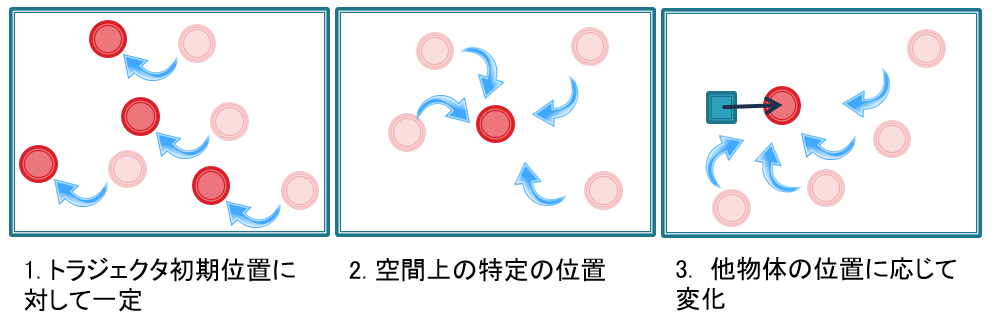
\includegraphics[width=14cm]{figure1.png} \\ %eXの基本として, \\ で緊急改行ができる。(今回の場合や行列などを除き、あまり使わない)
			\caption{トラジェクタ遷移の違い}
			\label{figure:moving_trajector}
		\end{center}
	\end{figure}
%%%%%%%%%%%%%%%%%%%%%%%%%%%%%%%%%%%%%%%%%%%%%%%%%%%%%%%%%%%%%%%%%%%%%%%%%%%%%%%%%%%%%%%%%%%%%%%%%%%%%%%
1はトラジェクタの初期位置を、2は画面中央を参照点に含めることで、3の特殊な事例として実現できる。即ち全ての物体移動動作は、参照点である物体位置、トラジェクタの初期位置、画面中央のうちいずれか一つ以上との相対位置を考慮した目標位置を持つ。

\subsection{変位}

特定の参照点に対し、動作はさらに以下の3種類が存在する。

	\begin{enumerate}
		\item 参照点を原点とし、常に一定の相対位置に遷移する
		\item 参照点を原点とし、トラジェクタの初期位置に応じて遷移先が変化する
		\item 複数の物体の位置関係に応じて遷移先が変化する
	\end{enumerate}
これら3種類の違いについてFig.\ref{figure:difference_displacement}で示す。
%%%%%%%%%%%%%%%%%%%%%%%%%%%%%%%%%%%%%%%%%%%%%%%%%%%%%%%%%%%%%%%%%%%%%%%%%%%%%%%%%%%%%%%%%%%%%%%%%%%%%%%
	\begin{figure}[t]
%中央ぞろえ
		\begin{center}
			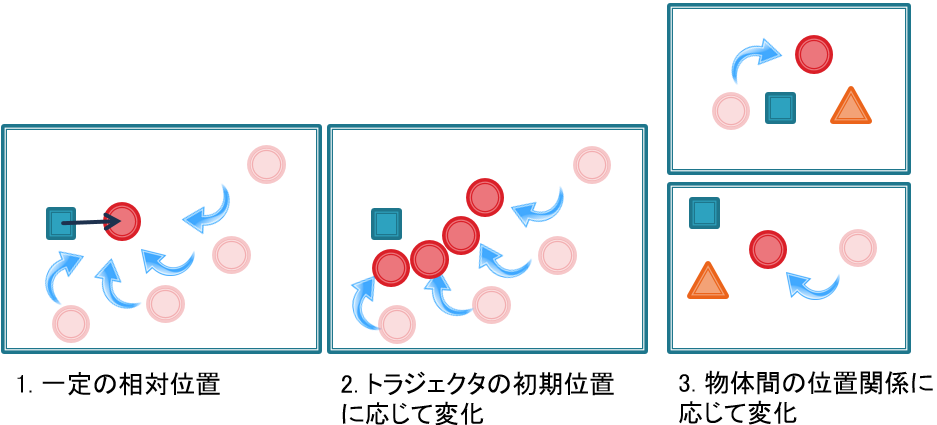
\includegraphics[width=14cm]{figure2.png} \\ %Teの基本として, \\ で緊急改行ができる。(今回の場合や行列などを除き、あまり使わない)
			\caption{参照点に対する遷移の違い}
			\label{figure:difference_displacement}
		\end{center}
	\end{figure}
%%%%%%%%%%%%%%%%%%%%%%%%%%%%%%%%%%%%%%%%%%%%%%%%%%%%%%%%%%%%%%%%%%%%%%%%%%%%%%%%%%%%%%%%%%%%%%%%%%%%%%%
1は例えばトラジェクタを物体の右隣に動かすという動作などで、参照点である物体に関して常に相対位置が一定である。2はトラジェクタを物体に近づけるという動作などで、これは参照点となる物体とトラジェクタの初期位置の位置関係によって、参照点からの目標位置の相対位置が変化する。3の例として、トラジェクタをある物体とある物体の間に動かすという動作などがあり、これは複数の物体を考慮した参照点の設定を行う必要がある。

\section{従来手法}

杉浦ら\cite{sugiura}の手法のアルゴリズムを以下に示す。(***これ以下、アルゴリズムはまだ書いてません***)

	\begin{algorithm}
		\caption{Algorithm of the conventional method(まだ途中)}
		\begin{algorithmic}
			\REQUIRE
				$N : the number of training data$ \\
				$M : the number of reference points$ \\
				$O : the number of objects$ \\
				$D = \{D_{1} , D_{2} , \ldots , D_{N}\} : training dataset$ \\
				$L = \{l_{1} , l_{2} , \ldots , l_{M}\} : the candidates of the reference point$ \\
		\end{algorithmic}
		\begin{algorithmic}[1]
			\IF{$n < 0$}
			\STATE $X \leftarrow 1 / x$
			\STATE $N \leftarrow -n$
			\ELSE
			\STATE $X \leftarrow x$
			\STATE $N \leftarrow n$
			\ENDIF
		\end{algorithmic}
	\end{algorithm}


杉浦らは参照点を各物体の位置、軌道開始点、画面中央に定め、座標系は原点の取り方、軸の向きの異なる数種類をあらかじめ設定し、最適な座標系および参照点を探索しながら、軌道に関する確率モデルである隠れマルコフモデルのパラメータを尤度最大化基準により学習する。この手法では参照点を各物体および軌道開始点、画面中央に限定しているため、複数の物体の位置関係を考慮した動作を学習できない。

\section{提案手法}

そのような問題点を踏まえ、提案手法では複数の参照点を学習に利用する手法を導入した。従来手法の拡張で複数の参照点を考慮できるようにするためには、参照点と変位(座標系)のいずれかに複数の参照点の情報を保持する機構を導入する必要がある。そこで参照点の候補に各参照点間の重心位置を採用することによって、参照点に複数の参照点の位置情報を含めることができると考えた。また本研究では物体移動動作を初期状態に対する最終状態の決定と定義し、動作中のトラジェクタ軌跡に関しては考えていないため、学習モデルはより単純なガウスモデルを使用した。
重心位置を参照点として考慮した際、構成する参照点同士の位置関係に対応した相対位置を学習するために、重心位置を原点として重心を構成する参照点の向きに軸を取る座標系を考慮する必要がある。そのため、重心位置に対する変位にはその構成参照点の数分の座標系を追加生成する。

\section{動作学習}

与えられた教示動作を用いて、各観点における確率モデルを更新し、学習を行う。以下に、提案手法の学習のアルゴリズムを示す。
	\begin{algorithm}[h]
		\caption{ Learning algorithm of the proposed method}
		\begin{algorithmic}
			\REQUIRE
				$N$ : the number of training data \\
				$M$ : the number of reference points , 
				$O$ : the number of objects \\
				$D = \{D_{1} , D_{2} , \ldots , D_{N}\}$ : training dataset \\
				$L = \{l_{1} , l_{2} , \ldots , l_{M}\}$ : the candidates of the reference point \\
				$K = \{k_{id} , k_{lt} , k_{gl}\}$ : coordinate systems \\
				$V = <L , K>$ : the candidates of the viewpoints \\
				$μ_{lk}$ : mean of the Probabilistic model of $<l , k>$ \\
				$Q_{lk}$ : mean-square of the Probabilistic model of $<l , k>$ \\
				$σ_{lk}$ : variance of the Probabilistic model of $<l , k>$ \\
				$T_{lk}(v)$ : Affine transfomation , 
				$F_{lk}(v)$ : Normalization
		\end{algorithmic}
		\begin{algorithmic}[1]
			\STATE$M \leftarrow 2^{O}$
			
			\FOR{$n=1$ to $N$}
				\STATE $d \leftarrow D_{n}$
				\FOR{$m=1$ to $M$}
					\FOR{all $k ∈K$}
						\STATE $d_{l_{m}k} \leftarrow F_{l_{m}k}(T_{l_{m}k}(d))$
						\STATE $μ_{l_{m}k} \leftarrow \frac{n-1}{n}μ_{l_{m}k} + \frac{1}{n}d_{l_{m}k}$
						\STATE $Q_{l_{m}k} \leftarrow \frac{n-1}{n}Q_{l_{m}k} + \frac{1}{n}(d_{l_{m}k})^2$
						\STATE $σ_{l_{m}k} \leftarrow Q_{l_{m}k} - (μ_{l_{m}k})^2$
					\ENDFOR
				\ENDFOR
			\ENDFOR
		\end{algorithmic}
	\end{algorithm}
ここで、$k_{id} , k_{lt} , k_{gl}$は座標系を表し、それぞれ画面に平行、参照点からトラジェクタの初期位置方向、参照点から重心の構成物体方向とする。参照点が複数の物体の重心でない場合、$k_{gl}$は考慮しない。また$F_{lk}(v)$は正規化関数を表し、次のように定める。
\[
	F_{lk}(v) = 
	\begin{cases}
		v & (if\,\,k=k_{id}) \\
		unit * \frac{v}{|v|} & (otherwise)
	\end{cases}
\]

$unit$は正規化長を表す。

\section{動作再現}

教示動作から学習された各観点における確率モデルを用いて、異なる初期環境での動作再現を行う。以下に、動作再現のアルゴリズムを示す。

\section{動作識別}

モデルが学習された各動作から例示動作の生起確率を計算することで、例示動作が既学習動作のうちいずれであるかを識別することが可能である。以下に、動作識別のアルゴリズムを示す。
